\documentclass{article}
\usepackage[utf8]{inputenc}
\usepackage[indonesian]{babel}

\title{Penggunaan Atribut Same-Site Cookies untuk Mencegah Serangan CSRF}
\author{Garin Ichsan Nugraha\\
Program Studi Sistem dan Teknologi Informasi\\
Sekolah Teknik Elektro dan Informatika\\
Institut Teknologi Bandung\\
Bandung, Indonesia\\
garin.kra@gmail.com}

\usepackage{natbib}
\usepackage{graphicx}
\usepackage{hyperref}
\usepackage{setspace}

\usepackage{listings}
\usepackage{color}


\definecolor{lightgray}{rgb}{0.95, 0.95, 0.95}
\definecolor{darkgray}{rgb}{0.4, 0.4, 0.4}
%\definecolor{purple}{rgb}{0.65, 0.12, 0.82}
\definecolor{editorGray}{rgb}{0.95, 0.95, 0.95}
\definecolor{editorOcher}{rgb}{1, 0.5, 0} % #FF7F00 -> rgb(239, 169, 0)
\definecolor{editorGreen}{rgb}{0, 0.5, 0} % #007C00 -> rgb(0, 124, 0)
\definecolor{orange}{rgb}{1,0.45,0.13}		
\definecolor{olive}{rgb}{0.17,0.59,0.20}
\definecolor{brown}{rgb}{0.69,0.31,0.31}
\definecolor{purple}{rgb}{0.38,0.18,0.81}
\definecolor{lightblue}{rgb}{0.1,0.57,0.7}
\definecolor{lightred}{rgb}{1,0.4,0.5}

\lstdefinelanguage{HTML5}{
  language=html,
  sensitive=true,	
  alsoletter={<>=-},	
  morecomment=[s]{<!-}{-->},
  tag=[s],
  otherkeywords={
  % General
  >,
  % Standard tags
	<!DOCTYPE,
  </html, <html, <head, <title, </title, <style, </style, <link, </head, <meta, />,
	% body
	</body, <body,
	% Divs
	</div, <div, </div>, 
	% Paragraphs
	</p, <p, </p>,
	% scripts
	</script, <script,
  % More tags...
  <canvas, /canvas>, <svg, <rect, <animateTransform, </rect>, </svg>, <video, <source, <iframe, </iframe>, </video>, <image, </image>, <header, </header, <article, </article
  },
  ndkeywords={
  % General
  =,
  % HTML attributes
  charset=, src=, id=, width=, height=, style=, type=, rel=, href=,
  % SVG attributes
  fill=, attributeName=, begin=, dur=, from=, to=, poster=, controls=, x=, y=, repeatCount=, xlink:href=,
  % properties
  margin:, padding:, background-image:, border:, top:, left:, position:, width:, height:, margin-top:, margin-bottom:, font-size:, line-height:,
	% CSS3 properties
  transform:, -moz-transform:, -webkit-transform:,
  animation:, -webkit-animation:,
  transition:,  transition-duration:, transition-property:, transition-timing-function:,
  }
}

\lstdefinestyle{htmlcssjs} {%
  % General design
%  backgroundcolor=\color{editorGray},
  basicstyle={\footnotesize\ttfamily},   
  frame=b,
  % line-numbers
  xleftmargin={0.75cm},
  numbers=left,
  stepnumber=1,
  firstnumber=1,
  numberfirstline=true,	
  % Code design
  identifierstyle=\color{black},
  keywordstyle=\color{blue}\bfseries,
  ndkeywordstyle=\color{editorGreen}\bfseries,
  stringstyle=\color{editorOcher}\ttfamily,
  commentstyle=\color{brown}\ttfamily,
  % Code
  language=HTML5,
  alsodigit={.:;},	
  tabsize=2,
  showtabs=false,
  showspaces=false,
  showstringspaces=false,
  extendedchars=true,
  breaklines=true,
  % German umlauts
  literate=%
  {Ö}{{\"O}}1
  {Ä}{{\"A}}1
  {Ü}{{\"U}}1
  {ß}{{\ss}}1
  {ü}{{\"u}}1
  {ä}{{\"a}}1
  {ö}{{\"o}}1
}

\lstset{style=htmlcssjs}

\onehalfspacing
\begin{document}

\begin{onehalfspacing}
\maketitle

\begin{abstract}
CSRF atau \textit{cross-site request forgery} adalah sebuah tindak kejahatan yang memanfaatkan penyimpanan kredensial pada suatu situs untuk mengeksekusi suatu perintah merugikan pada situs yang lainnya.Contohnya adalah penyerang yang membuat seseorang melakukan transfer ke rekening miliknya dengan memberikan suatu pranala yang akan mengeksekusi pengiriman uang dengan data kredensial yang telah disimpan dalam \textit{session} situs yang dibuka oleh pengguna atau biasa disebut dengan "\textit{cookies}". \textit{Cookies} sekarang sudah menjadi bagian yang sangat penting bagi setiap situs. \textit{Cookies} tidak hanya berfungsi untuk menyimpan informasi \textit{login} ataupun menyimpan kondisi situs pada saat tertentu. Pada kasus tertentu, \textit{cookies} dapat digunakan untuk \textit{web tracking}, analisis pengguna, dan periklanan daring dengan konsekuensi berkurangnya privasi pengguna yang digunakan untuk hal tersebut. Pada makalah ini akan dibahas tentang penggunaan \textit{same-site cookies} untuk mencegah terjadinya CSRF dan penerapannya sebagai perlindungan standar pada berbagai aplikasi penjelajah internet. \\

Kata Kunci: \textit{Same-Site}, \textit{Cookies}, CSRF, \textit{Security}.
\end{abstract}
\end{onehalfspacing}

\section{Pendahuluan}
Sekarang, penggunaan internet semakin umum dan meluas. Pada januari 2021, pengguna internet telah mencapai 4,46 Miliar, naik 7,7 persen dari tahun sebelumnya \cite{kemp_2021}. Internet banyak digunakan dengan berbagai kebutuhan manusia yang ada, terutama bisnis komersial. Semakin banyaknya penggunaan internet dalam bisnis komersial, akan semakin banyak juga pihak yang berusaha untuk menyerang dan mengambil keuntungan secara ilegal dengan memanfaatkan celah keamanan yang ada. Oleh karena itulah keamanan dalam internet, terutama bisnis komersial, merupakan hal yang sangat penting. 

Salah satu jenis serangan yang perlu kita khawatirkan adalah Cross-Site Request Forgery atau CSRF. Sebagian besar pengembang web tidak memiliki pengetahuan tentang serangan Cross Site Request Forgery (CSRF) yang merupakan kerentanan umum di antara berbagai serangan. Begitu pula dengan kebanyakan pengguna internet pada umumnya. Dalam serangan ini, korban dipaksa untuk melakukan tindakan yang tidak diinginkan di situs terpercaya, tanpa sepengetahuan dan tanpa interaksi pengguna \cite{sentamilselvan2013survey}. 

CSRF biasanya memanfaatkan kredensial yang tersimpan dalam peramban/penjelajah internet atau \textit{cookies} untuk mengeksekusi suatu perintah yang membutuhkan pengenalan \cite{sanchez2020cookies}. \textit{Cookies} HTTP adalah pecahan kecil data yang dapat dikirim peladen ke pengguna di dalam tanggapan mereka (dengan menggunakan \textit{Set-Cookieheader field}) atau dengan menggunakan kode JavaScript yang dieksekusi di halaman situs untuk membuat \textit{cookies} di sisi pengguna (dengan menjalankan \textit{document.cookiefunction}). Apa pun itu, peramban menyimpan nilai setiap \textit{cookies} dan menyertakannya di setiap permintaan masa depan yang dibuat ke peladen yang sama. Saat ini, \textit{cookies} digunakan untuk berbagai tujuan yang berbeda, termasuk untuk mempertahankan status \textit{login} pengguna, untuk menyimpan berbagai pilihan yang dibuat pengguna saat menjelajahi situs web (seperti preferensi bahasa atau penerimaan / penolakan persetujuan tertentu), atau untuk melacak kunjungan sebelumnya dari pengguna yang sama.


\begin{figure}[htbp]
    \centering
    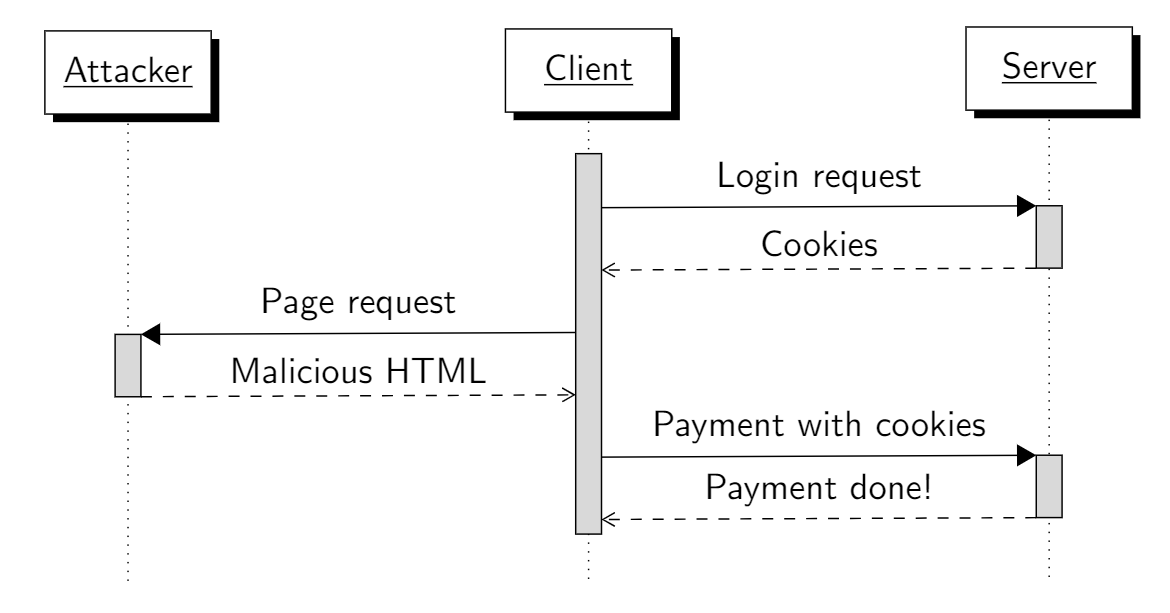
\includegraphics[scale=.5]{CSRF}
    \caption{Contoh CSRF \cite{calzavara2020security}}
    \label{fig:CSRF}
\end{figure}
Diagram \textit{use case} mengenai serangan CSRF pada Gambar 1 memberikan gambaran tentang bagaimana serangan CSRF dilakukan oleh penyerang. Situs web berbahaya dapat memaksa peramban situs pengguna untuk mengirim permintaan valid yang tidak sah ke situs yang ditargetkan. Contohnya seorang pengguna mengirim permintaan ke peladen untuk melihat halaman situs yang dibutuhkan kemudian peladen memberikan sesuai dengan permintaan. Namun pada saat tersebut, penyerang dapat saja memberikan suatu kode berbahaya yang diselipkan di halaman yang sama dalam \textit{tag} iframe atau \textit{tag} gambar, tetapi pengguna tidak memiliki pengetahuan bahwa pranala yang diselipkan di dalam kode akan mengarah ke halaman yang tidak diinginkan. Karena pengguna tidak terlalu tahu tentang tautan tersebut, dia dapat secara tidak sadar dipaksa untuk mengakses tautan tersebut dengan melakukan operasi klik pada tautan berbahaya tersebut. Sehingga secara tidak sadar, kode akan tereksekusi dan memaksa pengguna melakukan transaksi yang tidak diinginkan dengan memanfaatkan kredensial yang telah tersimpan di peramban pengguna. 

Pada makalah ini akan dibahas cara untuk mengatasi permasalahan CSRF tersebut. Terdapat sejumlah cara untuk mengatasi ancaman tersebut dan salah satunya adalah pemanfaatan \textit{same-site cookies}. Penggunaan \textit{same-site cookies} untuk mengatasi CSRF memiliki beberapa kekurangannya tersendiri. Akan tetapi, dengan beberapa penyesuaian tertentu, \textit{same-site cookies} menjadi salah satu pilihan yang mutakhir.

Makalah ini disusun dengan sistematika berikut. Pada bagian 2 terdapat contoh-contoh mengenai kejadian nyata serangan CSRF yang cukup besar dalam skalanya. Selanjutnya pada bagian 3 akan dijelaskan mengenai literatur terkait mengenai cara mengatasi serangan CSRF. Pada bagian 4 terdapat pembahasan yang akan menjelaskan secara detail mengenai CSRF, \textit{same-site cookie}, dan penerapan \textit{same-site cookie} untuk mengatasi serangan CSRF. Terakhir pada bagian ke-5 akan dijabarkan mengenai kesimpulan dari makalah ini.

\section{Contoh Nyata Serangan CSRF}
\subsection{ING Direct}
Ini adalah salah satu lembaga keuangan tempat serangan CSRF pertama kali terjadi \cite{zeller2008cross}. Serangan dilakukan dengan mentransfer dana keluar dari rekening bank pengguna oleh orang yang tidak berwenang. Ini karena kerentanan di situs web lNG. Serangan tersebut mengakibatkan sistem menambahkan akun tambahan atas nama pengguna yang sewenang-wenang.

\subsection{YouTube}
YouTube adalah salah satu situs yang paling banyak dikunjungi \cite{zeller2008cross}. Kerentanan di YouTube membuat orang yang tidak berwenang dapat menambahkan akun atas nama pengguna yang sah. Menggunakan akun yang telah didapatkan, penyerang tersebut menambahkan video ke "Favorit" pengguna, menambahkan dirinya sendiri ke daftar "Teman" atau "Keluarga" pengguna, mengirim pesan sewenang-wenang atas nama pengguna, menandai video sebagai tidak pantas, secara otomatis membagikan video dengan kontak pengguna, berlangganan pengguna ke "Channel" (sekumpulan video yang dipublikasikan oleh satu orang atau grup) dan menambahkan video ke "Quick List" pengguna (daftar video yang ingin ditonton pengguna di lain waktu).

\subsection{Metafilter}  
Metafilter adalah salah satu situs web yang mana kerentanan yang ada membuat akun pengguna dapat diambil alih oleh penyerang \cite{zeller2008cross}. Permintaan palsu dapat digunakan untuk menyetel alamat surel pengguna ke alamat penyerang. Permintaan palsu kedua kemudian dapat digunakan untuk mengaktifkan tindakan "Lupa Kata Sandi", yang akan mengirimkan kata sandi pengguna ke alamat surel penyerang. 

\subsection{The New York Times} 
Kerentanan yang ada di situs web The New York Times memungkinkan penyerang untuk mengetahui alamat surel dari pengguna secara sewenang-wenang \cite{zeller2008cross}. Serangan ini memanfaatkan fitur “Kirim ini lewat surel”  yang memungkinkan pengguna untuk mengirim surel tentang sebuah cerita ke pengguna yang sewenang-wenang. Surel ini akan berisi alamat surel pengguna. Penyerang dapat memalsukan permintaan untuk mengaktifkan fitur "Kirim ini lewat surel" sambil menyetel alamat surelnya sebagai penerima. Saat pengguna mengunjungi halaman penyerang, surel akan dikirim ke alamat surel penyerang dan berisi alamat surel pengguna. Serangan ini dapat digunakan untuk identifikasi (misalnya, menemukan alamat surel semua pengguna yang mengunjungi situs penyerang) atau untuk \textit{spam}. Serangan ini sangat berbahaya karena banyaknya pengguna yang memiliki akun NYTimes dan karena NYTimes membuat pengguna tetap masuk selama lebih dari setahun. Juga, Times People, situs jejaring sosial yang diluncurkan oleh New York Times pada 23 September 2008 , juga rentan terhadap serangan CSRF.

\subsection{GMail} 
Pada bulan Januari 2007, kerentanan serius ini ditemukan di GMail yang memungkinkan penyerang mencuri daftar kontak pengguna GMail \cite{siddiqui2011cross}.

\subsection{Nettlix}
Itu ditemukan di Nettlix yang memungkinkan penyerang untuk mengubah nama dan alamat pada akun, menambahkan film ke antrean sewa, dan sebagainya \cite{siddiqui2011cross}.

\subsection{EBay}  
EBay adalah salah satu situs lelang, di mana semakin banyak informasi disimpan. Serangan CSRF diterapkan yang mengakibatkan hilangnya banyak informasi pribadi sekitar 18 juta orang. Masalah ini ditemukan pada Februari 2008 \cite{alexenko2010cross}.

\subsection{Paypal} 
Pada 2016 terjadi serangan CSRF pada salah satu situs milik penyedia sistem pembayaran daring di sebagian besar negara yang mendukung transfer uang daring, dan berfungsi sebagai alternatif elektronik untuk metode kertas tradisional seperti cek dan wesel \cite{paypal_brook}. Dengan memanfaatkan kerentanan, hal terburuk yang dapat dilakukan seseorang adalah mengubah gambar profil pengguna lain. Tetapi karena halaman Paypal.me dapat digunakan dalam kapasitas profesional dan berfungsi sebagai profil publik bagi pengguna, akan jadi memalukan jika penyerang menggunakan kerentanan untuk mengubah gambar menjadi sesuatu yang tidak senonoh atau menyinggung.


\section{Literatur Terkait}
Ramarao R, Radhesh M, Alwyn R Pais \cite{ramarao2013preventing} menyajikan solusi \textit{proxy} sisi klien yang mendeteksi dan mencegah serangan CSRF menggunakan elemen IMG atau elemen HTML lain yang digunakan untuk mengakses gambar grafik untuk halaman situs. Proksi ini dapat memeriksa dan mengubah permintaan klien serta balasan (keluaran) aplikasi secara otomatis dan transparan memperluas aplikasi dengan teknik validasi token rahasia.

William Zeller dan Edward W. Felten \cite{zeller2008cross} menerapkan \textit{plugin} peramban sisi klien yang dapat melindungi pengguna dari jenis serangan CSRF tertentu. Mereka menerapkan alat mereka sebagai ekstensi ke peramban situs Firefox. Pengguna perlu mengunduh dan menginstal ekstensi ini agar efektif melawan serangan CSRF. Ekstensi mereka bekerja dengan mencegat setiap permintaan HTTP dan memutuskan apakah itu harus diizinkan. Keputusan ini dibuat dengan menggunakan aturan berikut. Pertama, permintaan apa pun yang bukan merupakan permintaan POST diperbolehkan. Kedua, jika situs yang meminta dan situs target berada di bawah kebijakan asal yang sama, permintaan tersebut diizinkan. Ketiga, jika situs yang meminta diizinkan untuk membuat permintaan ke situs target menggunakan kebijakan lintas domain Adobe, permintaan tersebut diizinkan. Jika ekstensi mereka menolak permintaan, ekstensi memberitahu pengguna bahwa permintaan telah diblokir menggunakan antarmuka yang sudah dikenal (yang sama digunakan oleh pemblokir \textit{popup} Firefox) dan memberi pengguna opsi untuk menambahkan situs ke \textit{white list}.

Sooel Son \cite{son2010prevent} mengusulkan \textit{Prevent Cross-site Request Forgery attack} (PCRF). PCRF adalah skema pertahanan yang menghasilkan token dinamis terhadap CSRF. Tujuan dasar PCRF adalah untuk mencegah serangan CSRF dengan menambahkan token baru ke setiap permintaan situs yang halaman targetnya harus dilindungi secara satu arah agar efisien mencegah serangan CSRF terhadap aplikasi situs PHP. PCRF memberikan solusi otomatis yang kuat terhadap ancaman CSRF dengan menggunakan token CSRF. Karena properti fungsi \textit{hash} yang aman secara kriptografis, hal ini juga digunakan untuk memverifikasi apakah token telah dikeluarkan sebelumnya dari peladen.

Nanad jovanovic et.al \cite{jovanovic2006preventing} mengusulkan mekanisme mitigasi untuk CSRF yang hanya memberikan perlindungan parsial dengan mengganti permintaan POST dengan permintaan GET atau mengandalkan informasi di \textit{header Referer} dari permintaan HTTP dan juga mengusulkan solusi yang menyediakan perlindungan otomatis lengkap dari Serangan XSRF. Lebih tepatnya, pendekatannya didasarkan pada \textit{proxy} sisi peladen yang mendeteksi dan mencegah serangan CSRF dengan cara yang transparan bagi pengguna serta aplikasi situs itu sendiri (\textit{proxy ortogonal}).

Johns dan Winter \cite{johns2006requestrodeo} memperkenalkan RequestRodeo, solusi sisi klien untuk melawan ancaman ini. Dengan pengecualian SSL sisi klien, RequestRodeo menerapkan perlindungan terhadap eksploitasi mekanisme otentikasi implisit. Perlindungan ini dicapai dengan menghapus informasi otentikasi dari permintaan yang mencurigakan. Mereka mengusulkan solusi sisi klien untuk memungkinkan pengguna yang sadar keamanan melindungi diri mereka dari serangan CSRF. Solusi mereka berfungsi sebagai \textit{proxy} lokal di komputer pengguna.

\section{Pembahasan}
\subsection{CSRF}
Cross-Site Request Forgery (CSRF) adalah serangan yang memaksa \textit{end user} untuk melakukan tindakan yang tidak diinginkan pada aplikasi situs tempat mereka saat ini diautentikasi \cite{csrf_owasp}. Dengan sedikit bantuan manipulasi psikologis (seperti mengirim tautan melalui surel atau obrolan), penyerang dapat mengelabui pengguna aplikasi situs untuk menjalankan tindakan yang dipilih penyerang. Jika korbannya adalah pengguna biasa, serangan CSRF yang berhasil dapat memaksa pengguna untuk melakukan permintaan perubahan status seperti mentransfer dana, mengubah alamat surel, dan lain sebagainya. Jika korbannya adalah akun administratif, CSRF dapat membahayakan seluruh aplikasi situs.

\begin{figure}[htbp]
    \centering
    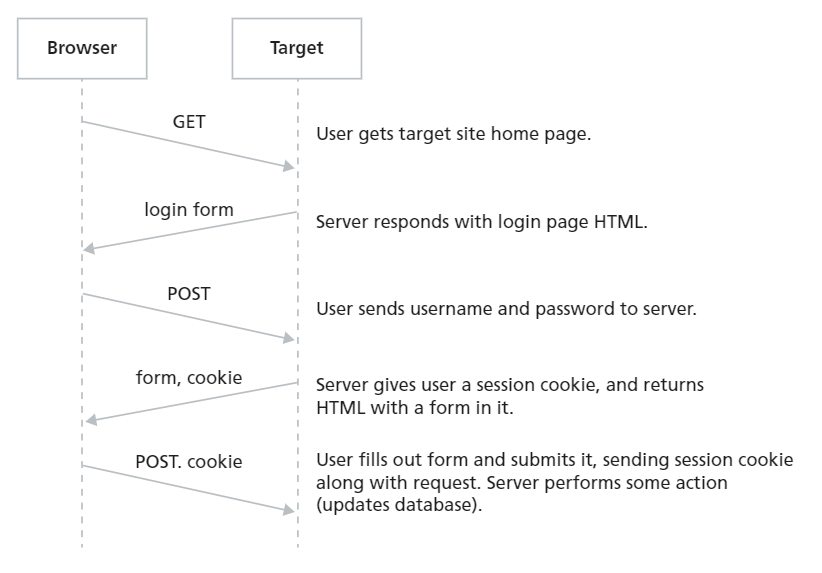
\includegraphics[scale=.6]{normal visit}
    \caption{Kejadian normal dalam mengunjungi sebuah situs}
    \label{fig:normal}
\end{figure}

Untuk mengetahui lebih jelas, lihat pada Gambar 2 yang merupakan penjelasan peristiwa yang terjadi ketika kita mengunjungi situs pada umumnya \cite{blatz2007csrf}. Pada Gambar 3 merupakan peristiwa yang terjadi ketika terdapat serangan CSRF. Dari sudut pandang peladen situs, tidak ada yang aneh dengan permintaan POST kedua. Formatnya bagus, dan berisi sesi \textit{cookies} yang valid. Secara naif, peladen situs akan memproses permintaan tersebut.

\begin{figure}[htbp]
    \centering
    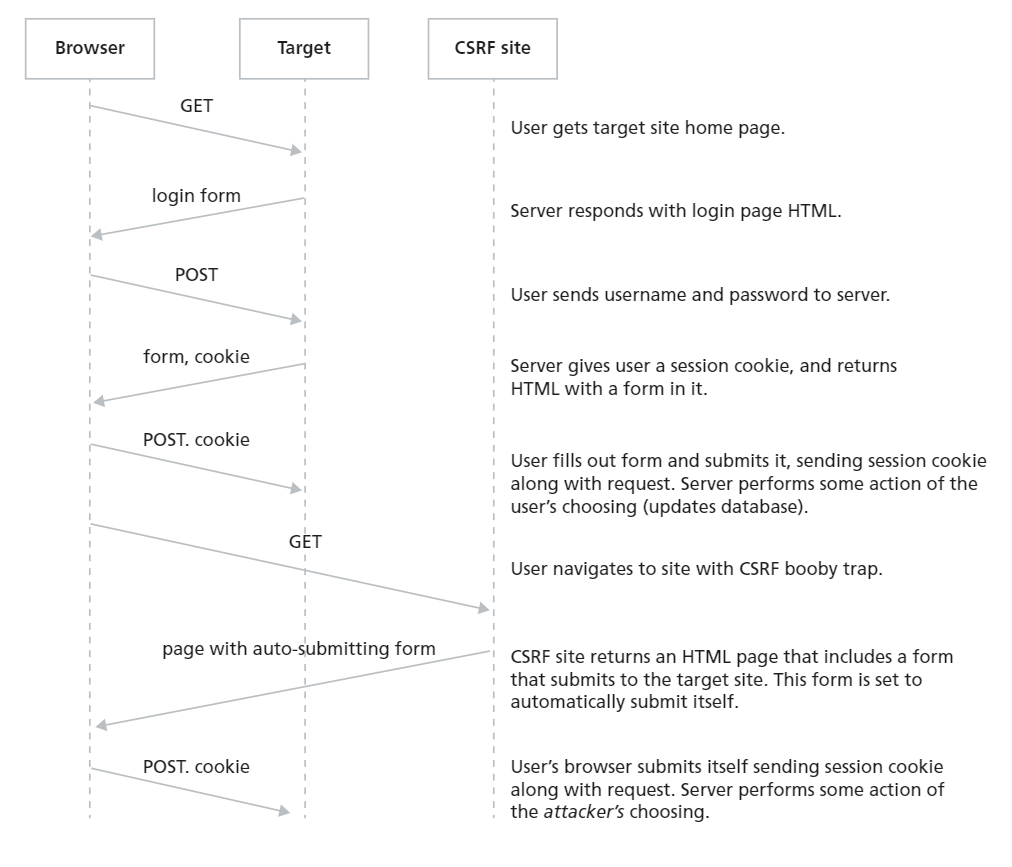
\includegraphics[scale=.5]{csrf attack}
    \caption{Serangan CRSF dalam sebuah situs}
    \label{fig:attack}
\end{figure}

\subsubsection{Sifat Serangan}
Berikut adalah sifat-sifat utama dalam serangan CSRF \cite{blatz2007csrf}.
\begin{itemize}
\item \textbf{Korban tidak perlu "\textit{login}" }(bergantung pada tujuan penyerang)

Meskipun tujuan CSRF yang paling umum adalah memanfaatkan otentikasi korban untuk melakukan beberapa tindakan yang diautentikasi, CSRF dapat digunakan untuk berbagai serangan. Misalnya, penyerang mungkin menggunakan CSRF untuk melakukan tindakan curang dan tidak diautentikasi, seperti memberikan suara dalam jajak pendapat daring. Atau, penyerang mungkin meluncurkan serangan \textit{denial-of-service} (DoS) menggunakan CSRF, dengan memposting pesan di papan pesan populer yang membuat permintaan-permintaan ke situs lain. Terakhir, CSRF dapat digunakan untuk menyalahgunakan hubungan kepercayaan yang tidak aman antara penjajah dan peladen situs, seperti situs yang menggunakan batasan alamat IP, otentikasi dasar HTTP, atau sertifikat klien SSL.
\item \textbf{Penyerang dapat membuat permintaan dari serangkaian permintaan apa pun di situs target}

Dengan kata lain, tidak peduli berapa banyak langkah yang diperlukan untuk tindakan tersebut; penyerang dapat membuat skrip beberapa permintaan
\item \textbf{CSRF bekerja sangat baik dengan serangan lain}

Melakukan tindakan yang valid di situs target bisa sangat berguna bagi penyerang. CSRF juga dapat digunakan dengan serangan lain untuk membuat skenario "\textit{death by a thousand cuts}". Beberapa contohnya adalah menggunakan CSRF untuk mengeksploitasi skrip lintas situs paska-otentikasi atau serangan injeksi SQL, atau untuk mengeksploitasi skrip lintas situs yang hanya dapat dieksploitasi melalui HTTP POST.
\item \textbf{Penyerang biasanya tidak dapat membaca data dari situs target}

Meskipun CSRF adalah alat yang ampuh untuk penyerang, namun penggunaanya sangat terbatas. Karena \textit{same-origin policy}, skrip di satu situs tidak dapat membaca data dari skrip di situs lain. Oleh karena itu, tindakan \textit{multi-step} yang mana hasil dari satu langkah harus dimasukkan ke langkah berikutnya biasanya kebal dari CSRF. Tentu saja ada pengecualian untuk aturan ini. 

Misalnya, jika keluaran yang disebutkan di atas dapat diprediksi, penyerang mungkin dapat menebak atau melakukan  \textit{brute-force}. Selain itu, jika ada kerentanan \textit{single cross-site scripting} di situs target, maka semuanya dibatalkan. Penyerang mungkin dapat memanfaatkan skrip lintas situs untuk meluncurkan serangan baca-tulis terhadap target. Mungkin juga ada kasus lain yang mana penyerang mungkin dapat membaca beberapa data dari situs target.
\end{itemize}

\subsubsection{Jenis Serangan}
Sebagai contoh, situs korban adalah \textit{target.example.com} memiliki halaman di dalamnya, \textit{form.html}, yang mengirimkan datanya ke \textit{action.html} \cite{blatz2007csrf}. Dalam penggunaan yang sah, pengguna akan memuat \textit{http://target.example.com/form.html}, mengisi data di formulir, lalu menekan tombol kirim. perambannya kemudian akan mengirim permintaan ke \textit{http://target.example.com/action.html}, yang akan melakukan beberapa tindakan menggunakan data tersebut.
\begin{enumerate}
\item \textbf{\textit{Inline “image” links}}

Serangan CSRF dapat dilakukan dengan beberapa cara. Yang paling sederhana adalah menyematkan referensi ke sumber daya eksternal (misalnya, gambar) di halaman lain. Serangan ini sangat mudah diluncurkan, karena hampir semua situs papan buletin memungkinkan pengguna untuk menyematkan gambar di unggahan mereka. Ingatlah bahwa peramban tidak memiliki cara untuk mengetahui bahwa "gambar" yang diminta sebenarnya adalah halaman situs yang melakukan beberapa tindakan. Sebagai contoh, unggahan berikut di papan pesan akan menyebabkan browser mengirim permintaan ke peladen situs target.
\begin{lstlisting}[style=htmlcssjs]
I agree with the above poster
<img src="http://target.example.com/action.html?field1=foo&field2=bar" width="1" height="1">
\end{lstlisting}

\item \textbf{Auto-submitting forms}

Jika tindakan tersebut membutuhkan HTTP POST, serangannya sedikit lebih kompleks. Penyerang dapat membuat formulir menggunakan HTML atau JavaScript. Ini memerlukan penyerang untuk memiliki beberapa tingkat kendali atas situs CSRF, karena mereka harus menyematkan HTML mereka sendiri di situs. Mereka dapat memperoleh kontrol ini baik dengan menjadi pemilik situs atau dengan menemukan semacam kerentanan skrip lintas situs di situs tersebut. Sayangnya, menemukan situs web dengan kerentanan skrip lintas situs sangatlah mudah; persentase situs dengan kerentanan skrip lintas situs diperkirakan sangat tinggi — hingga 70 hingga 80 persen. Berikut adalah contoh yang menggunakan formulir HTML di situs penyerang.
\begin{lstlisting}[language=HTML]
<html>
 <body onload="document.frames[0].submit()"">
     <form action="http://target.example.com/action.html" method="POST">
        <input name="field1" value="foo">   <input name="field2" value="bar">  
     </form> 
 </body>
</html>
\end{lstlisting}
Penyerang akan memasukkan yang berikut ini ke dalam situs CSRF:
\begin{lstlisting}[language=HTML]
<iframe width="0" height="0" style="visibility: hidden;" src="http://attacker.example.com/CSRF.html">
\end{lstlisting}
Penggunaan skrip lintas situs juga dapat digunakan untuk menyebabkan halaman tidak berbahaya di situs CSRF bertindak sebagai halaman berbahaya. Dengan kata lain, situs apa pun di Internet dengan kerentanan skrip lintas situs dapat digunakan untuk meluncurkan serangan CSRF. Ini membebaskan penyerang dari keharusan menjadi tuan rumah di halaman serangannya sendiri.
\item \textit{\textbf{Phishing}}

Cara termudah untuk mengeksploitasi CSRF, dari sudut pandang teknis, adalah memiliki kendali penuh atas situs CSRF dan kemudian meyakinkan korban Anda untuk mengunjungi situs tersebut. \textit{Phishing} bisa sangat berguna untuk serangan berskala besar dan bertarget.

Untuk serangan skala besar terhadap bank konsumen dan sejenisnya, pelaku \textit{phising} dapat melengkapi informasi mereka dengan tindakan aktual di situs target. Bahkan jika korban menolak memberikan informasi mereka, mereka mungkin sudah memiliki rencana cadangannya.

Untuk serangan yang ditargetkan, \textit{phishing} bahkan lebih efektif. Sistem intranet dan administratif adalah target CSRF yang sangat baik, dan penyerang dapat menyesuaikan surel \textit{phishing}-nya untuk target tersebut. Misalnya, jika menyerang intranet, \textit{phisher} dapat mengirim surel yang mengaku dari mitra pelatihan perusahaan atau penyedia asuransi. Jika menyerang blog, \textit{phisher} dapat mengirim surel kepada pengelola tentang situs yang keren. Jika menyerang sistem \textit{helpdesk}, \textit{phisher} dapat mengirim surel ke dukungan tentang masalah pada situs tersebut. Korban tidak perlu melakukan tindakan apa pun di situs CSRF, mengunjungi situs saja sudah cukup. Selain itu, di sebagian besar contoh ini, korban memiliki peluang yang sangat besar untuk terkelabuhi saat menerima surel \textit{phishing}.

\end{enumerate}

\subsubsection{Kemampuan Serangan}
Seperti yang telah dijelaskan sebelumnya, serangan CSRF memungkinkan penyerang mengirim permintaan HTTP ke situs pihak ketiga menggunakan peramban situs korban. Itu merupakan jaring yang cukup besar. Di bawah ini adalah beberapa contoh spesifik. Ingatlah bahwa situs target dapat berupa situs apa pun yang dapat diakses dari peramban korban \cite{blatz2007csrf}. Ini termasuk situs intranet dan situs lain yang bahkan tidak dapat diakses dari Internet.
\begin{enumerate}
\item \textbf{Mensimulasikan permintaan yang sah}

Ketika orang berbicara tentang serangan CSRF, biasanya inilah yang mereka maksud. Penyerang menggunakan CSRF untuk melakukan tindakan normal secara curang di situs target. Tindakan mungkin termasuk: 
\begin{itemize}
\item Mengubah alamat surel pengguna dan kemudian melakukan operasi "lupa kata sandi Anda" untuk mendapatkan akses ke akun pengguna 
\item Menambahkan akun untuk blog pengguna atau sistem lain 
\item Mentransfer dana dari rekening bank pengguna 
\item Melakukan pembelian atau memesan stok sebagai bagian dari skema "\textit{pump and dump}" 
\item Memeriksa keberadaan berkas.Ini dapat digunakan untuk mencari dan sidik jari peladen situs di intranet.
\end{itemize}
\item \textbf{Mengaktifkan XSS, injeksi SQL}

Di luar operasi normal, CSRF dapat digunakan untuk mengeksploitasi kerentanan di situs target. Saat memprioritaskan remediasi, pemilik situs sering kali tidak memprioritaskan skrip lintas situs pada sistem administratif dan intranet, serangan XSS yang hanya dapat dieksploitasi melalui POST HTTP, dan injeksi SQL di bagian situs yang hanya dapat diakses oleh pengguna tepercaya. Dengan CSRF, semua ini pada dasarnya rentan terhadap penyerang yang tidak terautentikasi.
\item \textbf{Memanggil layanan situs}

Dalam beberapa kasus, serangan CSRF dapat memanggil layanan situs. Dengan menggunakan atribut "\textit{enctype}" dari formulir HTML, penyerang dapat mengirimkan XML semi-valid ke titik akhir layanan situs, misalnya:
\begin{lstlisting}
<form action="http://target.example.com/webservice" method="POST" enctype="text/plain">
    <input name="<msg><attr><name>a</name><value>b</value></attr></msg>" value="">
    <input type="submit">
</form>
\end{lstlisting}
Satu-satunya kekurangan untuk ini adalah bahwa penyerang tidak dapat mengatur \textit{header} permintaan, sehingga permintaan ke layanan situs SOAP (yang memerlukan \textit{header} "SOAPAction") tidak akan berfungsi.
\end{enumerate}

\subsection{\textit{Same-site Cookies}}
Atribut \textit{SameSite} pada \textit{cookies} menyediakan tiga cara berbeda untuk mengontrol perilaku ini. Anda dapat memilih untuk tidak menentukan atribut, atau Anda dapat menggunakan "\textit{Strict}" atau "\textit{Lax}" untuk membatasi \textit{cookies} ke permintaan situs yang sama \cite{SameSite9:online}. Jika Anda menyetel \textit{SameSite} ke \textit{Strict}, \textit{cookie} Anda hanya akan dikirim dalam konteks pihak pertama. Dalam istilah pengguna, \textit{cookie} hanya akan dikirim jika situs untuk \textit{cookie} cocok dengan situs yang saat ini ditampilkan di bilah URL peramban. Jadi, jika \textit{cookie promo shown} disetel sebagai berikut:
\begin{lstlisting}
Set-Cookie: promo_shown=1; SameSite=Strict
\end{lstlisting}

Ketika pengguna berada di situs Anda, maka \textit{cookie} akan dikirim dengan permintaan seperti yang diharapkan. Namun ketika mengikuti tautan ke situs Anda, katakanlah dari situs lain atau melalui surel dari teman, atas permintaan awal itu \textit{cookie} tidak akan dikirim. Ini akan bagus jika Anda memiliki \textit{cookie} yang berkaitan dengan fungsionalitas yang akan selalu berada di belakang navigasi awal, seperti mengubah sandi atau melakukan pembelian, tetapi akan terlalu membatasi untuk \textit{promo shown}. Jika pembaca Anda mengikuti tautan ke situs, mereka ingin \textit{cookie} mereka dikirim sehingga preferensi mereka dapat diterapkan. 

Di situlah \textit{SameSite = Lax} yang mengizinkan \textit{cookie} dikirim dengan navigasi tingkat atas ini digunakan. Mari kita lihat contoh artikel kucing berikut yang mana situs lain mereferensikan konten Anda. Mereka menggunakan foto kucing Anda secara langsung dan memberikan tautan ke artikel asli Anda.
\begin{lstlisting}
<p>Look at this amazing cat!</p>
<img src="https://blog.example/blog/img/amazing-cat.png" />
<p>Read the <a href="https://blog.example/blog/cat.html">article</a>.</p>
\end{lstlisting}

Saat pembaca berada di blog orang lain, \textit{cookie} tidak akan dikirim saat browser meminta \textit{amazing-cat.png}. Namun ketika pembaca mengikuti tautan ke cat.html di blog Anda, permintaan itu akan menyertakan \textit{cookie}. Ini menjadikan \textit{Lax} pilihan yang baik untuk \textit{cookie} yang memengaruhi tampilan situs dan \textit{Strict} berguna untuk cookie yang terkait dengan tindakan yang diambil pengguna Anda. 

Terakhir, ada opsi untuk tidak menentukan nilai yang sebelumnya telah menjadi cara untuk menyatakan secara implisit bahwa Anda ingin \textit{cookie} dikirim dalam semua konteks. Ini dibuat eksplisit dengan memperkenalkan nilai baru dari \textit{SameSite = None}. Ini berarti Anda dapat menggunakan "None" untuk menyampaikan dengan jelas bahwa Anda sengaja ingin \textit{cookie} dikirim dalam konteks pihak ketiga. Untuk dapat lebih memahami ketiga cara tersebut, lihat Gambar 4 yang menggambarkan bagaimana penggunaan ketiga cara tersebut pada konteks suatu \textit{cookie}.
\begin{figure}[htbp]
    \centering
    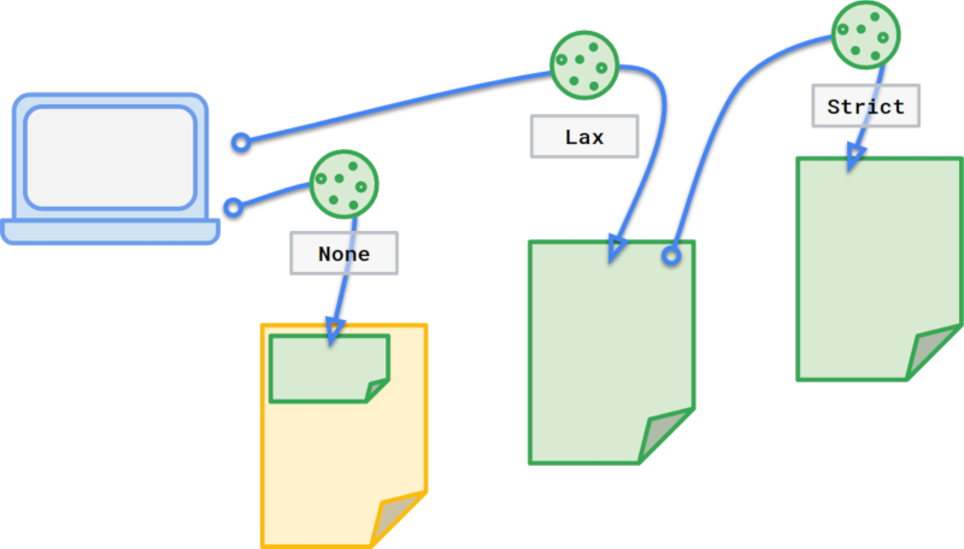
\includegraphics[scale=.3]{cookie context}
    \caption{Menandai konteks \textit{cookie} secara eksplisit sebagai \textit{None}, \textit{Lax}, atau \textit{Strict}}
    \label{fig:cookiecontext}
\end{figure}

\textit{Same-site cookie} memiliki kelebihan dan kekurangannya tersendiri. Kelebihannya adalah dapat berjalan di berbagai aplikasi tanpa perlu melakukan pengubahan kode secara drastis. Selain itu, tingkat keketatannya dapat kita atur dengan tingkat \textit{strict}, \textit{lax}, dan \textit{none} sesuai dengan kebutuhan situs. Sedangkan kekurangannya adalah \textit{cookie} ini belum didukung oleh beberapa peramban situs lama \cite{CanIuseS40:online,ietf-httpbis-rfc6265bis-07}. Cookie ini juga berkemungkinan untuk konflik dengan \textit{single sign-on cookie-based} sehingga \textit{single sign-on} tidak dapat digunakan tanpa pengaturan tambahan terlebih dahulu.

\subsection{Penerapan}
Secara default, \textit{same-site cookies} tidak akan dikirim bersama dengan navigasi tingkat atas \cite{ietf-httpbis-cookie-same-site-00}. Penggunaan \textit{cookie} ini bisa jadi kompatibe ataupun tidak kompatibe dengan sistem manajemen sesi yang ada. Untuk menyediakan mekanisme \textit{drop-in} yang mengurangi risiko serangan CSRF, pengembang dapat menyetel atribut "\textit{SameSite}" dalam mode "\textit{Lax}" yang membuat pengecualian yang mengirimkan \textit{cookie} situs yang sama bersama dengan permintaan lintas situs jika dan hanya jika itu adalah navigasi tingkat atas yang menggunakan metode HTTP yang "aman".

Penggunaan "Lax" memberikan pertahanan yang wajar dan mendalam terhadap serangan CSRF yang mengandalkan metode HTTP yang tidak aman (seperti "POST"), tetapi tidak menawarkan pertahanan yang kuat terhadap CSRF sebagai kategori serangan umum:
\begin{enumerate}
\item Penyerang masih dapat memunculkan jendela baru atau memicu navigasi tingkat atas untuk membuat permintaan "\textit{same-site}" yang hanya merupakan \textit{speedbump} dalam melakukan eksploitasi.
\item Fitur seperti "<link rel = 'prerender'>" atau prapenguraian dapat dimanfaatkan untuk membuat permintaan "\textit{same-site}" tanpa risiko terdeteksi oleh pengguna.
\end{enumerate}

Beberapa peramban sudah mulai menerapkan sistem keketatan "Lax" pada atribut \textit{same-site cookie} sebagai sebuah pengaturan utama \cite{calzavara2020security}. Google Chrome mengambil inisiatif pertama untuk menerapkannya pada versi ke-80 mereka. Jika seorang pengembang belum mau untuk menerapkannya, pengembang dapat menerapkan tingkat keketatan "None" secara eksplisit untuk menimpa pengaturan otomatis tersebut. Yang perlu diperhatikan adalah \textit{cookie} harus ditandai sebagai "\textit{Secure}" untuk dapat tetap beroperasi.
\section{Kesimpulan}
\textit{Same-site cookie} dapat diterapkan pada suatu situs untuk mencegah terjadinya serangan \textit{cross-site request forgery}. Penerapan yang paling disarankan untuk penggunaan secara umum adalah dengan tingkat keketatan "\textit{Lax}". Tingkat keketatan "Strict" ataupun "None" juga dapat digunakan sesuai dengan tingkat keamanan yang kita butuhkan. Seorang pengembang harus mengetahui tentang pengaturan atribut tersebut untuk dapat mengamankan kredensial dari pengguna atau bahkan \textit{administrator} dari suatu situs itu sendiri.

Meskipun \textit{same-site cookie} memiliki beberapa kekurangan dalam pengaplikasiannya. Kekurangan tersebut masih dapat diatasi dengan sedikit pengaturan tambahan. Jika dibandingkan dengan keuntungan yang didapatkan maka hal tersebut adalah suatu hal yang bermanfaat untuk dilakukan. Beberapa peramban situs juga sudah mulai menerapkan tingkat keketatan "\textit{Lax}" sebagai pengaturan utama atribut \textit{same-site cookie} mereka. Hal ini tentunya mendorong para pengembang untuk dapat mengaplikasikannya lebih lanjut.

\bibliographystyle{plain}
\begin{onehalfspacing}
\bibliography{references}
\end{onehalfspacing}

\end{document}
